\subsection{Route-Specific Lifecycles and Evidence}
\label{sec:routes}
\label{sec:mech}
\label{sec:objective}
\label{sec:nodeexec}
\label{sec:ack}

\paragraph{Timing and approval}
Timing guards are route-specific. Online node writes enforce an effective
minimum spacing of 60\,s. Recipe dispatch uses a per-recipe interval anchored
to approval, while trials also use a configurable per-line cadence (default
300\,s). The recipe interval can refuse a proposal before an approval request
is created. Checks occur at proposal or execution according to the operation,
and experiment-specific pacing overrides are reported with the corresponding
results.

Manual bindings create an approval request containing the actor, node or
recipe, candidate values, applicable limits, expiry, and parameter bases.
The default wait expires after 180\,s and refuses execution. After approval,
the executor rechecks authorization and active limits to account for context
changes during the wait. For \texttt{recipe\_apply}, a changed definition
requires a new proposal; an unchanged approval dispatches a copy of the
approved parameter snapshot. A line-level recipe mode defaults to manual;
changing it to automatic requires administrator confirmation. The approval
record authorizes a workflow action and does not replace process protection.

\begin{figure*}[!t]
\centering
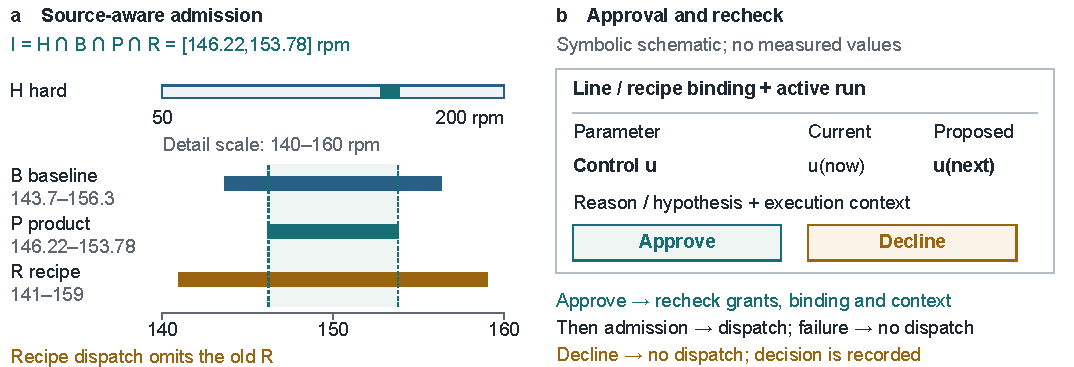
\includegraphics[width=\textwidth]{resources/fig-admission-hitl-2026.pdf}
\caption{Admission and approval boundaries. (a) Archived Q1 RPM example:
online node interventions use the four-layer value interval of Eq.~(1),
whereas recipe dispatch omits the prior recipe window. (b) Symbolic human
approval binds a proposed action and authority fields; execution checks run
again after approval, which does not reserve equipment state.}
\label{fig:hitl}
\end{figure*}

\paragraph{Node probe}
The bounded node probe is exposed as \texttt{optimization\_explore} to the
Auto Modeling Lab (AML) optimization profile (\texttt{aml\_optimization}).
The profile validates a bound control and target DAQ scope,
captures a starting control and target baseline, invokes the internal DCW
write path, then waits 10--300\,s (default 45\,s) and queries a trailing 45-s
target window before saving an exploration summary. Since each window is
relative to its query time, approval can separate baseline sampling from
actuation; a 10-s wait can leave about 35\,s of pre-write samples in the later
window. The command receipt and target summary are therefore returned
separately. A successful changed-value write opens a node-optimization
record; refusal or expired approval creates a rejected summary without a
post-write sample.

\paragraph{Recipe operations}
\texttt{recipe\_trial} checks the bound recipe and active run, then dispatches
candidate overrides as a batch with per-parameter verification. The caller
subsequently queries DAQ and decides whether to save a new definition with
\texttt{recipe\_update}, restore one with \texttt{recipe\_rollback}, or
dispatch a version with \texttt{recipe\_apply}. These steps are separate: a
trial does not save or apply a version, and endpoint verification is not a
process-response measurement. Public direct-node control is closed; the
bounded probe and recipe operations are the configured operation surfaces.
The historical four-scene results use an earlier direct-node path and do not
test current profile or binding adaptation across scenes.

\paragraph{Command verification}
Command confirmation and process response answer different questions. A
driver ACK is graded as \texttt{readback-verified}, \texttt{transport-ack},
or \texttt{unverified}. A matching endpoint read supports the first grade; a
transport or MES application receipt supports the second. Recipe batch
verification assigns \texttt{verified}, \texttt{unverified}, or
\texttt{failed}; if no matching readback is available, it attempts up to
three independent reads, 2\,s apart. A matching retry upgrades the final ACK,
while exhausted retries remain unverified. The initial ACK remains in write
history and the final ACK and verdict are retained with the batch.
Per-parameter receipts preserve successful outcomes when another parameter
fails. A readback-verified setpoint does not establish target attainment.

\paragraph{Observation, verdict, and compensation}
The caller performs recipe-path observation after batch dispatch. The October
recipe case therefore compares a recipe definition, endpoint readback, and
DAQ sample as separate representations. Saving a definition, applying it to
equipment, and observing its process response are separately evidenced
operations. The evaluation does not combine these route-specific records into
one universal end-to-end record.

An open node record provides a monitoring backstop. After 120\,s it polls
every 30\,s; three cumulative samples outside the recipe monitoring window
trigger a system-attributed rollback request toward the preceding value.
Missing samples do not count as breaches. A caller's \texttt{keep},
\texttt{rollback}, or \texttt{uncertain} verdict records its interpretation;
compensation is a new command subject to its applicable admission policy.
The write audit deduplicates the same value on the same node within 10\,s,
while batch receipts, exploration summaries, DAQ history, and recipe versions
retain their distinct lifecycles. Linking these records by actor and
production context allows the command, endpoint evidence, and process
observation to be inspected without treating them as interchangeable.
\label{sec:agentloop}
